\documentclass{llncs}

\newif\ifnoTBD \noTBDfalse

% Uncomment to remove TBD macros
%\noTBDtrue

\ifx\pdftexversion\undefined
  \usepackage[dvips]{graphicx}
\else
  \usepackage[pdftex]{graphicx}
  \usepackage{epstopdf}
\fi

\ifnoTBD
\def\TBD#1{\typeout{TBD not done: #1}}
\else
\def\TBD#1{\textcolor{blue}{TBD: #1}}
\AtEndDocument{\typeout{ *** ATTENTION: compilation is in DRAFT
    mode. There might still be TBD that appear in the document ***}}
\fi

\usepackage[usenames]{color}
\usepackage{xspace}
\usepackage{listings}
\usepackage{url}
\usepackage{latexsym}
\usepackage{comment}
\usepackage{color}
\usepackage[table]{xcolor}
\usepackage{amsfonts} 
\usepackage{amssymb,amsmath} 
\usepackage[strings]{underscore}

\newcommand{\ompi}{Open\,MPI\xspace}
\newcommand{\abft}{Algorithmic Based Fault Tolerance\xspace}
\newif\ifulfmsaid
\newcommand{\ulfm}{\ifulfmsaid ULFM\else User-Level Failure Mitigation (ULFM)\ulfmsaidtrue\fi\xspace}
\newcommand{\mpifunc}[1]{{\tt #1}}

\begin{document}

\title{User Level Failure Mitigation in MPI}
\author{Wesley Bland}
\institute{Innovative Computing Laboratory, University of Tennessee\\
           \email{wbland@eecs.utk.edu}}

\maketitle

%\begin{abstract}

As recent research has demonstrated, it is becoming a necessity for large scale
applications to have the ability to tolerate process failure during an
execution. As the number of processes increases, checkpoint/restart fault
tolerance approaches requiring large concurrent state checkpointing become untenable and radically new
methods to address fault tolerance are needed. This work addresses these
challenges by proposing a novel approach to a minimalistic fault discovery and
management model.  Such a model allows application to run to
completion despite fail-stop failures. As a proof of concept, in addition to the
proposed fault tolerance model, an implementation in the context of the \ompi
library is provided, evaluated and analyzed.
% as well as providing a corresponding implementation in the context of the
% \ompi project.  allow applications to discover and tolerate failures while
% continuing execution, all while minimizing application involvement. It
% includes modifications to the \ompi runtime as well as MPI library to give the
% user options when deciding how best to implement fault tolerance.

\end{abstract}


\section{Motivation} \label{sect:intro}

Fault tolerance is an increasingly necessary consideration in High Performance Computing (HPC). As machine sizes increase past hundreds of thousands of computing cores\footnote{http://www.top500.org} into the millions of computing resources, the likelihood of failures also increases. Observed failures rates are reaching between 1.8 and 3.6 failures per day on a system of only 635 nodes. This research confirms what has become an accepted reality of HPC going forward. Failures will occur at an increasing rate and for large scale applications to be useful, the failures will need to be handled in software while allowing the applications to continue running relatively uninterrupted.

This realization has lead to much research to attempt to solve the problems presented by the necessity for fault tolerance. The first and most well understood form of fault tolerance is rollback-recovery using periodic checkpointing. This form of fault tolerance has been widely adopted and works well for small scale machines where failure rates are expected to be relatively low. However, at larger scales, even with more reliable hardware, the  time spent performing checkpointing operations is expected to exceed the amount of time spent performing useful computation. To resolve this problem, we turn to Application Based Fault Tolerance (ABFT).

ABFT changes the way applications recover from failure. Rather than loading a previous checkpoint from disk and restarting an entire application, the algorithm itself recovers from the loss of a process and continues without the need to perform costly, large-scale checkpointing operations. The exact method used to recover from failures changes from application to application, but all applications have some requirements in common. The programming model and environment, together with the supporting runtime, need to provide basic functionality in order to allow applications to build a comprehensive fault management solution.

This is a challenging requirement. Most applications continue to use message passing to perform communication between processes, and in the message passing paradigm, collective communication is a popular and necessary way for groups of processes to communicate efficiently. However, collective communication also creates problems when trying to maintain the functionality of the communication library following a process failure due to the complex communication patterns and topologies that must be repaired. 

In addition to maintaining a functional communication library with scalable fault tolerance mechanisms, a fault tolerance solution must also provide extensibility. Because ABFT takes different forms for different applications, the fault tolerance provided by the communication library should also be able to adapt. For example, while one type of application may work best with a transactional model of fault tolerance where sections of the application are re-executed when recovery is necessary, a master-slave type of application may choose to simply spawn a replacement for any process which fails and continue on without needing further recovery.

To this end, we have modified a runtime system to support two new forms of fault tolerance within the message passing paradigm which can provide a suite of tools necessary for developers to include resilience in their applications. Due to size restrictions, details on the work implementing a resilient runtime can be found in~\cite{Bland:CCGrid12}.
%\section{Related Work}
\label{sect:related}

Efforts toward fault tolerance in MPI have previously been attempted.  Automatic
fault tolerance~\cite{Bouteiller10Redesign,MPICHVblocking} is a compelling
approach for users, as failures are completely masked and handled internally by
the MPI library, which requires no new interfaces to MPI or application code
changes. Unfortunately, many recent studies point out that automatic approaches,
either based on checkpoints or replication, will exhibit poor efficiency on
Exaflop platforms~\cite{BOSILCA-2012-696154,lawn265}.

Application Based Fault Tolerance
(ABFT)~\cite{fthpl2011,pengduppopp12,huang1984algorithm} is another approach
that promises better scalability, at the cost of significant algorithm and 
application code changes. Despite some limited 
successes~\cite{europar12/onfailureckpt,Gropp:2004:FTM:1080704.1080714},
MPI interfaces need to be extended to effectively support ABFT. The most notable past 
effort is FT-MPI~\cite{fagg2000ft}, which provided several recovery modes for the user 
but was never standardized and therefore was not portable enough for most users.
\section{Motivation}
\label{sect:motivation}

A major concept followed in the design of any type of parallel programming paradigm, and
this in order to provide a meaningful and understandable programming approach,
is the avoidance of any potential deadlocks. In addition to this critical
requirement the mechanisms involved in the fault management were build with the
goal of flexibility, simplicity and performance.

Clearly the most important point, no MPI call (point-to-point or collective) can
block indefinitely after a failure, but must either succeed or raise an MPI
error. Fault tolerance at the application level is impossible if the application
cannot regain full control of the execution after a process failure. The MPI
library must guarantee that it will automatically stabilize itself following a
process failure, and provide the tools necessary for the application to resolve
its own deadlock scenarios on an application specific basis.
% The \ulfm proposal implements this idea with the \mpifunc{MPI\_COMM\_REVOKE}
% construct, detailed in Section~\ref{sect:newmpi}.

Second, the API should allow varied fault tolerant models to be built. MPI has
been conceived with the goal of portability and extendability, and have been
constructed to support libraries leveraging existing MPI constructs to create
more abstractions or tighter integration with libraries. Maintaining this design
strength was paramount for \ulfm, and it provides this capability so other
levels of consistency can be supported as needed by higher-level
concepts. Transactional fault tolerance, strongly uniform collective operations,
and other FT techniques can all therefore be built upon the proposed set of
constructs.

An API should be easy to understand and use in common scenarios, as complex
tools have a steep learning courve and a slow adoption by the targeted
communities. To this end, the number of newly proposed constructs have been
reduced to five (along with nonblocking variants). These five functions provide
the minimal set of tools to implement fault tolerant applications and libraries.

Two major pitfalls must be avoided when implementing these concepts: jitter
prone, permanent monitoring of the health of peers a process is not actively
communicating with, and expensive consensus required for returning consistent
errors at all ranks.  The operative principle is that fault-related errors are
local knowledge, and are not indicative of the return status on remote
processes. Errors are raised at a particular rank, when based on local knowledge
it is known that a particular operation cannot complete because a participating
peer has failed.

\section{New MPI Constructs}
\label{sect:newmpi}

This section succinctly presents the prominent interfaces proposed
to enable effective support of User-Level Failure Mitigation for MPI
applications. The interested reader can refer to the technical document
for a complete description of the interfaces~\cite{BlandULFMTechReport}
and to the amended standard draft\footnote{http://svn.mpi-forum.org/trac/mpi-forum-web/ticket/323}.

Designing the mechanism that users would use to manage failures was built around
three concepts: 1) simplicity, the API should be easy to understand
and use in most common scenarios; 2) flexibility, the API should allow
varied fault tolerant models to be built as external libraries and; 3) absence
of deadlock, no MPI call (point-to-point or collective) can block
indefinitely after a failure, but must either succeed or raise an MPI error.
Two major pitfalls must be avoided: jitter prone, permanent 
monitoring of the health of peers a process is not actively
communicating with, and expensive consensus required for returning
consistent errors at all ranks. The operative principle is then that
errors (\mpifunc{MPI\_ERR\_PROC\_FAILED}) are not indicative of the
return status on remote processes, but are raised only at a particular
rank, when a particular operation cannot complete because a participating 
peer has failed. The following functions 
provide the basic blocks for maintaining consistency and enabling 
recovery of the state of MPI.

\paragraph{\mpifunc{MPI\_COMM\_FAILURE\_ACK} \& \mpifunc{MPI\_COMM\_FAILURE\_GET\_ACKED}:}\label{sect.ack}

These two calls allow the application to determine which processes within a
communicator have failed. The acknowledgement function serves to mark a point in
time which will be used as a reference. The function to get the acknowledged
failures refers back to this reference point and returns the group of processes
which were locally known to have failed.
After acknowledging failures, the application can resume
\mpifunc{MPI\_ANY\_SOURCE} point-to-point
operations between non-failed processes, but operations involving failed
processes (such as collective operations) will likely continue to raise errors.

\paragraph{\mpifunc{MPI\_COMM\_REVOKE}:}

Because failure detection is not global to the communicator, some
processes may raise an error for an operation, while others do not. This
inconsistency in error reporting may result in some processes continuing
their normal, failure-free execution path, while others have diverged to
the recovery execution path. As an example, if a process, unaware of the
failure, posts a reception from another process that has switched to the
recovery path, the matching send will never be posted. Yet no failed 
process participates in the operation and it should
not raise an error. The receive operation is effectively deadlocked.
The revoke operation provides a mechanism for the application to resolve such
situations before entering the recovery path. A revoked communicator becomes
improper for further communication, and all future or pending communications on
this communicator will be interrupted and completed with the new error code
\mpifunc{MPI\_ERR\_REVOKED}. It is notable that although this operation is not
collective (a process can enter it alone), it affects remote ranks without a
matching call.

\paragraph{\mpifunc{MPI\_COMM\_SHRINK}:}

The shrink operation allows the application to create a new communicator by
eliminating all failed processes from a revoked communicator. The operation is
collective and performs a consensus algorithm to ensure that all participating
processes complete the operation with equivalent groups in the new communicator.
This function cannot return an error due to process failure. Instead, such errors
are absorbed as part of the consensus algorithms and will be excluded from the
resulting communicator.

\paragraph{\mpifunc{MPI\_COMM\_AGREE}:}

This operation provides an agreement algorithm which can be used to determine a
consistent state between processes when such strong consistency is
necessary. The function is collective and forms an agreement over a boolean
value, even when failures have happened or the communicator has been
revoked. The agreement can be used to resolve a number of consistency issues
after a failure, such as uniform completion of an algorithmic phase or
collective operation, or as a key building block for strongly consistent failure
handling approaches (such as transactions).

\section{Implementation Issues}
\label{sect:algorithms}

\begin{comment}

In this section, we detail the challenges and advantages of the aforementioned
MPI constructs. They unfold along three main axes, the amount of supplementary
state and memory to be kept within the MPI library, the additional operations to
be executed on the critical path of communication routines, and the algorithmic
cost of failure recovery routines. We discuss, in general, options available to
implementors, and highlight issues with insight from a prototype implementation
in Open~MPI~\cite{gabriel04:_open_mpi}.

\subsection{Impact on communication routines}

\paragraph*{Memory:} Because a communicator cannot be repaired,
tracking the state of failed processes imposes a minimal memory overhead.  From
a practical perspective each node needs a global list of detected failures,
shared by all communicators; its size grows linearly with the number of
failures, and it is empty as long as no failures occur.  Within each
communicator, the supplementary state is limited to two values: whether the
communicator is revoked or not, and an index in the global list of failures
denoting the last acknowledged failure (with
\mpifunc{MPI\_COMM\_FAILURE\_ACK}). For efficiency reasons, an implementation
may decide to cache the fact that some failures have happened in the
communicator so that collective operations and \mpifunc{MPI\_ANY\_SOURCE}
receptions can bail out quickly. Overall, the supplementary memory consumption
from fault tolerant constructs is small, independent of the total number of
nodes, and unlikely to affect the cache and TLB hit rates.

\paragraph*{Conditionals:} Another concern is the number of supplementary
conditions on the latency critical path. Indeed, most completion operations
require a supplementary conditional statement to handle the case where the
underlying communication context has been revoked. However, the prediction
branching logic of the processor can be hinted to favor the failure free
outcome, resulting in a single load of a cached value and a single, mostly
well-predicted, branching instruction, unlikely to affect the instruction
pipeline. It is notable that non-blocking operations raise errors related to
process failure only during the completion step, and thus do not need to check
for revocation before the latency critical section.

\paragraph*{Matching logic:} \mpifunc{MPI\_COMM\_REVOKE} does not have a
matching call on other processes on which it has an effect. As such, it might
add detrimental complexity to the matching logic. However, any MPI
implementation needs to handle unexpected messages. The order of revocation
message delivery is loose enough that the handling of revocation notices can be
integrated within the existing unexpected message matching logic. In our
implementation in Open~MPI, we leverage the active message low level transport
layer to introduce revocation as a new active message tag, without a single
change to the matching logic.

\paragraph*{Collective operations:} A typical MPI implementation supports a
large number of collective algorithms, which are dynamically selected depending
on criteria such as communicator or message size and hardware topology. The
loose requirements of the proposal concerning error reporting of process
failures in collective operations limits the impact it has on collective
operations. Typically, the collective communication algorithms and selection
logic are left unchanged. The only new requirement is that failures happening at
any rank of the communicator cause all processes to exit the collective
(successfully for some, with an error for others). Due to the underlying
loosely-connected topologies used by some algorithms, a point-to-point based
implementation of a collective communication is unlikely to detect all process
failures.  Fortunately, a practical implementation exists that does not require
modifying any of the collective operations: when a rank raises an error because
of a process failure, it can revoke an internal, temporary communication
context associated with the collective operation. As the revocation notice
propagates on the internal communicator, it interrupts the point-to-point
operations of the collective. An error code is returned to the high level MPI
wrapper, which in turn raises the appropriate error on the user's communicator.

\subsection{Recovery routines}

\end{comment}

Some of the recovery routines described in Section~\ref{sect:newmpi} are
unique in their ability to deliver a valid result despite the occurrence
of failures. This specification of correct behavior across failures calls
for resilient, more complex algorithms. In most cases, these functions
are intended to be called sparingly by users, only after actual failures have
happened, as a means of recovering a consistent state across all
processes. This section describes the algorithms that
can be used to deliver this specification and their cost. 
An evaluation of the failure-free impact on implementations can be found in~\cite{Bland:2012tp}.

\paragraph*{Agreement:}
\label{subsect:agreement}

The agreement can be conceptualized as a failure-resilient reduction on
a boolean value. Many agreement algorithms have been proposed in the 
literature; the log-scaling two-phase consensus algorithm used by the \ulfm
prototype is one of many possible implementations of
\mpifunc{MPI\_COMM\_AGREE} operation based upon prior work in the field.
Specifically, this algorithm is a variation of the multi-level two-phase
commit algorithms~\cite{Mohan_1985}. A more extensive discussion of the
algorithm and its complexity has been published by Hursey,
et.al.~\cite{Hursey11LogConsensus}.

\paragraph*{Revoke:}
\label{subsect:revoke}

A concern with the revoke operation is the number of supplementary
conditions introduced to the latency critical path. Indeed, most completion operations
require a supplementary conditional statement to handle the case where the
underlying communication context has been revoked. However, the prediction
branching logic of the processor can be hinted to favor the failure free
outcome, resulting in a single load of a cached value and a single, mostly
well-predicted, branching instruction, unlikely to affect the instruction
pipeline. It is notable that non-blocking operations raise errors related to
process failure only during the completion step, and thus do not need to check
for revocation before the latency critical section.

\paragraph*{Shrink:} The Shrink operation is, algorithmically, an agreement on
which the consensus is done on the group of failed processes.
Hence, the two operations have the same algorithmic complexity. Indeed, in the
prototype implementation, \mpifunc{MPI\_COMM\_AGREE} and
\mpifunc{MPI\_COMM\_SHRINK} share the same internal implementation of the
agreement.

\section{Performance Analysis}
\label{sect:performance}

The following analysis used a prototype of the \ulfm proposal based on
the development trunk of Open MPI~\cite{gabriel04:_open_mpi} (r26237).
The test results presented were gathered from the Smoky system at Oak
Ridge National Laboratory. Each node contains four quad-core 2.0~GHz AMD
Opteron processors with 2 GB of memory per compute core. Compute nodes
are connected with gigabit Ethernet and InfiniBand. Some shared-memory
benchmarks were conducted on Romulus, a $6\times8$-core AMD Opteron 6180
SE with 256GB of memory (32GB per socket) at the University of Tennessee.

\begin{figure}[ht]
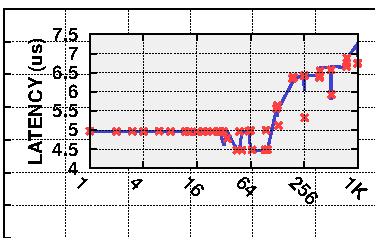
\includegraphics[width=.49\textwidth]{figures/np-ibsmoky}
\hfill
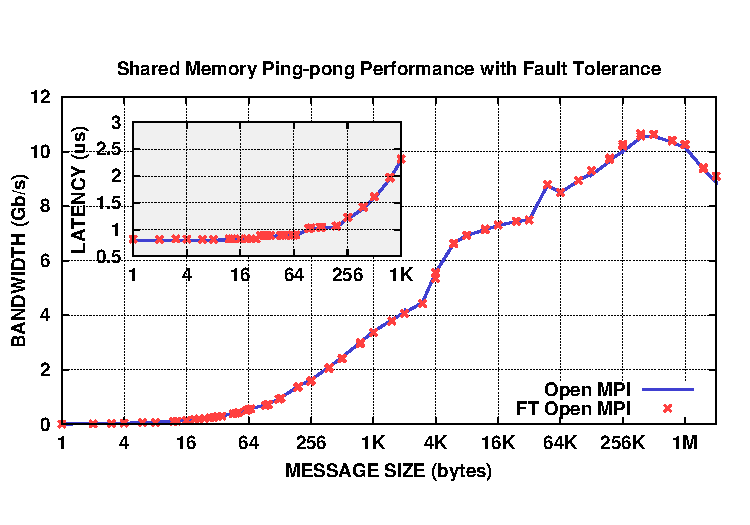
\includegraphics[width=.49\textwidth]{figures/np-smsmoky}
\caption{Netpipe Latency and Bandwidth Impact of Enabling Fault Tolerance Support (on Smoky)\label{fig:netpipe}.}
\end{figure}

\begin{table}%\vspace{-.4cm}
\begin{center}\sf\scriptsize
\begin{tabular}{|l||r|r||r|r||r|}
\multicolumn{6}{c}{1-byte Latency (microseconds) (cache hot)} \\
\hline
\cellcolor[gray]{0.7}\textbf{Interconnect}  & \cellcolor[gray]{0.7}\textbf{Vanilla}   & \cellcolor[gray]{0.7}\textbf{Std. Dev.} &
\cellcolor[gray]{0.7}\textbf{FT}            & \cellcolor[gray]{0.7}\textbf{Std. Dev.} & \cellcolor[gray]{0.7}\textbf{Difference} \\
\hline
\cellcolor[gray]{0.9}Shared Memory &  0.8008 & 0.0093 &  0.8016 & 0.0161 &  0.0008 \\
\cellcolor[gray]{0.9}TCP           & 10.2564 & 0.0946 & 10.2776 & 0.1065 &  0.0212 \\
\cellcolor[gray]{0.9}OpenIB        &  4.9637 & 0.0018 &  4.9650 & 0.0022 &  0.0013 \\
\hline
\multicolumn{6}{c}{Bandwidth (Mbps) (cache hot)} \\
\hline
\cellcolor[gray]{0.7}\textbf{Interconnect}  & \cellcolor[gray]{0.7}\textbf{Vanilla}   & \cellcolor[gray]{0.7}\textbf{Std. Dev.} &
\cellcolor[gray]{0.7}\textbf{FT}            & \cellcolor[gray]{0.7}\textbf{Std. Dev.} & \cellcolor[gray]{0.7}\textbf{Difference} \\
\hline
\cellcolor[gray]{0.9}Shared Memory &  10,625.92 &  23.46 &  10,602.68 & 30.73 & -23.24 \\
\cellcolor[gray]{0.9}TCP           &   6,311.38 &  14.42 &   6,302.75 & 10.72 &  -8.63 \\
\cellcolor[gray]{0.9}OpenIB        &   9,688.85 &   3.29 &   9,689.13 &  3.77 &   0.28 \\
\hline
\end{tabular}
\end{center}
\caption{Standard Deviation of the NetPIPE results (on Smoky).\label{tab:netpipe}}%\vspace{-.8cm}
\end{table}

The NetPIPE benchmark (v3.7) was used to assess the 1-byte latency and
bandwidth impact of the modifications necessary for the \ulfm support in
\ompi. We compare the vanilla version of \ompi (r26237) with the \ulfm
enabled version on Smoky (labelled as FT). Figure~\ref{fig:netpipe} compares the
bandwidth and latency achieved by these two builds of \ompi. As can be
observed, for the entire range of message sizes, the performance
difference is insignificant, either when using the Infiniband network
transport, or with the most stressful shared-memory transport.
Table~\ref{tab:netpipe} presents the standard deviation across 100 runs,
and further highlights the fact that the differences in performance are
not only well below the noise limit, but that the standard deviation
difference is negligible, thus proving the performance stability and
lack of impact.


\begin{figure}[ht]
\begin{center}%\vspace{-.6cm}
 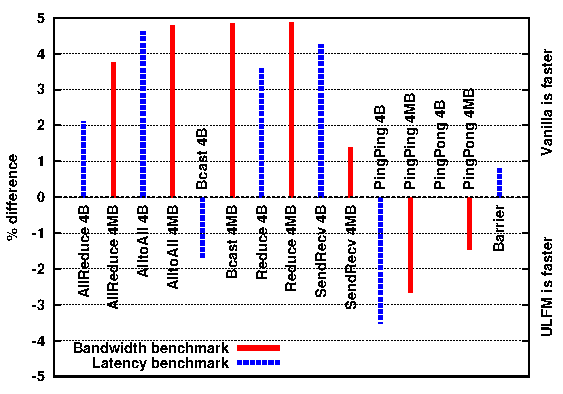
\includegraphics[width=.7\linewidth]{figures/IMB.pdf}%\vspace{-.4cm}
 \caption{The Intel MPI Benchmarks: relative difference
   between \ulfm and the vanilla Open MPI on shared memory
  (Romulus). Standard deviation $\approx$5\% on 1,000 runs.\label{fig:IMB}}%\vspace{-.6cm}
\end{center}
\end{figure}

The impact on shared memory systems, which are sensitive even to small
modifications of the MPI library, has been further assessed on the
Romulus machine -- a large shared memory machine -- using the IMB
benchmark suite (v3.2.3). As shown in Figure~\ref{fig:IMB}, the duration
difference of all the benchmarks (point-to-point and collective) remains
below 5\%, thus within the standard deviation of the implementation on
that machine.

To measure the impact of the prototype on a real application, we used the
Sequoia AMG benchmark\footnote{https://asc.llnl.gov/sequoia/benchmarks/\#amg}.
This MPI intensive benchmark is an Algebraic Mult-Grid (AMG) linear system
solver for unstructured mesh physics. A weak scaling study was conducted up to
512 processes following the problem \emph{Set 5}. In
Figure~\ref{fig:sequoia:bargraph}, we compare the time slicing of three main
phases (Solve, Setup, and SStruct) of the benchmark, with, side by side, the
vanilla version of the Open MPI implementation, and the \ulfm enabled one. The
application itself is not fault tolerant and does not use the features proposed
in \ulfm. The goal of this benchmark is to demonstrate that a careful
implementation of the proposed semantic does not impact the performance of the
MPI implementation, and ultimately leaves the behavior and performance
of legacy applications unchanged. The results show that the performance 
difference is negligible.

\begin{figure}[ht]
\centering
    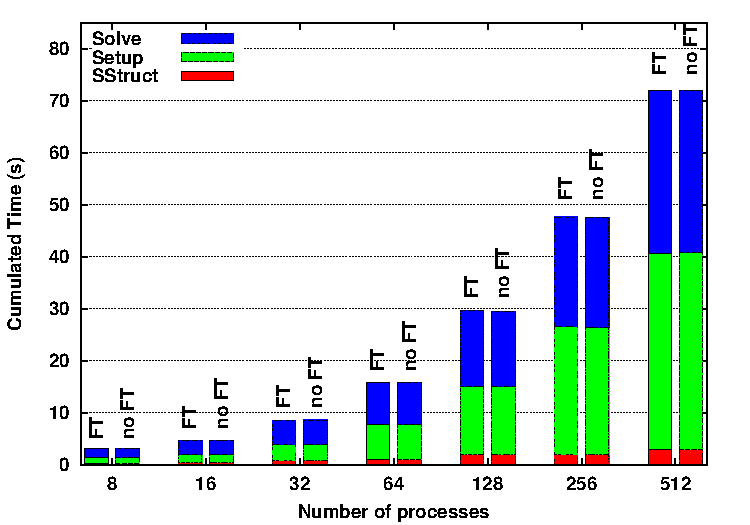
\includegraphics[width=.7\linewidth]{figures/bargraph.pdf}%\vspace{-.4cm}
    \caption{Comparison of the vanilla and \ulfm versions of Open MPI running
      Sequoia-AMG at different scales (Smoky).\label{fig:sequoia:bargraph}}
\end{figure}
\begin{figure}[ht]
\centering
    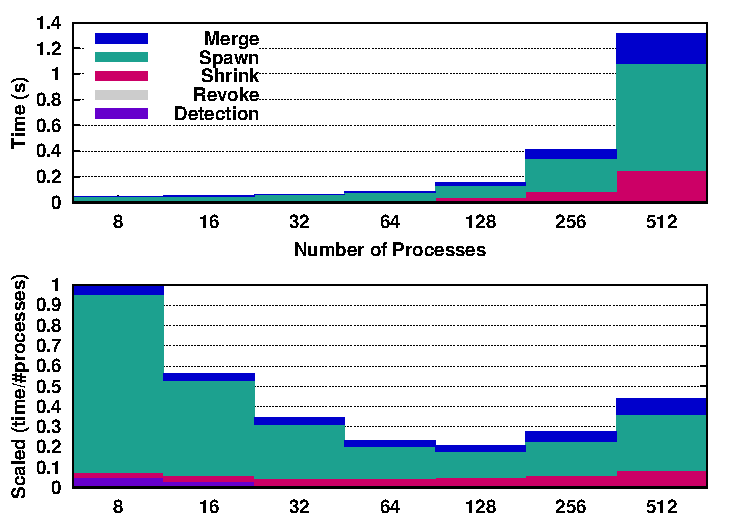
\includegraphics[width=.7\linewidth]{figures/repair.pdf}%\vspace{-.4cm}
    \caption{Evaluation of the Fault Injection Benchmark with full
      recovery at different scales (Smoky).\label{fig:frssj:scalability}The top graph presents absolute times, the bottom graph presents the same results divided by the number of processes, to form a composite unit that better highlights scalability trends.}
\end{figure}

To assess the overheads of recovery constructs, we developed a synthetic
benchmark that mimics the behavior of a typical fixed-size tightly-coupled
fault-tolerant application. Unlike a normal application it performs an infinite
loop, where each iteration contains a failure and the corresponding recovery
procedure. Each iteration consists of 5 phases: in the first phase
(\emph{Detection}), all processes but a designated victim enter a Barrier on the
intracommunicator. The victim dies, and the failure detection mechanism makes
all surviving processes exit the Barrier, some with an error code. In Phase 2
(\emph{Revoke}), the surviving processes that detected a process-failure related
error during the previous phase invoke the new construct
\mpifunc{MPI\_COMM\_REVOKE}. Then they proceed to Phase 3 (\emph{Shrink}) where
the intracommunicator is shrunk using \mpifunc{MPI\_COMM\_SHRINK}. The two
other phases serve to repair a full-size intracommunicator using MPI-2
spawn and intercommunicator merge operations to allow the
benchmark to proceed to the next round.

In Figure~\ref{fig:frssj:scalability}, we present the timing of each phase,
averaged upon 50 iterations of the benchmark loop, for a varying number of
processes on the Smoky machine. 
%We focus on the three points related to \ulfm:
%failure detection, revoke and shrink. 
The scaled graph presents the same result, but scaled down accordingly
 to the number of processors used; the resulting normalized unit is 
irrelevant, but improves readability for small deployments and  
better highlight scalability trends. 

The failure detection is mildly impacted by the scale. In the prototype
implementation, the detection happens at two levels, either in the
runtime system or in the MPI library (when it occurs on an active link).
Between the two detectors, all ranks get notified within 30ms of the
failure (this compares to the 1s timeout at the link level).

Although the revoke call injects a logarithmic number of messages (to
different targets) in the network to implement the level of reliability
required for this operation, the duration of this call itself is under
50$\mu$s and is not visible in the figure. The network is disturbed for
a longer period, due to the processing of the messages, but this
disturbance will appear in the network only after a failure occurred.
According to the performance of the next operation (Shrink), this
disturbance has no practical consequences.

The duration of the new construct to shrink a communicator behaves
similarly to other communicator manipulation operations (as illustrated
by comparing with the intercomm merge operation). Indeed, the Shrink
operation includes two operations, one is the agreement on the group of
failed processes, the second one is the allocation of a new communicator
identifier (an operation that also appears in intercomm merge). Because
in this benchmark, no new failure disrupts the (shrink-internal)
agreement operation, it completes in the same time as a regular
collective communication would. Consequently, a significant portion of
the time of the Shrink operation is spent in the underlying communicator
creation functions (unmodified from MPI-2).

The Spawn operation, directly inherited from MPI-2, and left unmodified
in the \ulfm prototype, exhibits poor performance and scalability. The
reason is mostly historical: \mpifunc{MPI\_COMM\_SPAWN} has seen little
use in the past, and thereby has not been the focus of intensive
optimizations from implementors. Should the use of this construct become
more ubiquitous, it is expected that a careful implementation would
reach adequate performance, for it is not prevented by theoretical
difficulties.

An interesting observation is that all three operations Shrink, Spawn,
an Merge pay for the cost of the allocation of a communicator
identifier; an overhead that appears to be significant at scale. This
suggests that the \ulfm specification could benefit from the addition of
an operation realizing these three operations at once, thereby dividing
this overhead by three.

\section{Conclusion}
\label{sect:conclusion}

Many responsible voices agree that sharp increases in the volatility of future,
extreme scale computing platforms are likely to imperil our ability to use them
for advanced applications that deliver meaningful scientific results and
maximize research productivity. Since MPI is currently, and will likely continue
to be -- in the medium-term -- both the de-facto programming model for
distributed applications and the default execution model for large scale
platforms running at the bleeding edge, it is the place in the software
infrastructure where semantic and run-time support for application faults needs
to be provided.

The \ulfm proposal is a careful but important step forward toward accomplishing
this goal delivering support for a number of new and innovative resilience
techniques through simple, familiar API calls, but it is backward compatible
with previous versions of the MPI standard, so that non fault-tolerant
applications (legacy or otherwise) are supported without any changes to the
code. Perhaps most significantly, applications can use \ulfm-enabled MPI without
experiencing any degradation in their performance, as we demonstrate in this
paper. Some of these applications along with other portable libraries are
currently being refactored to take advantage of \ulfm semantics.

The author would like to acknowledge his co-authors in the full
paper~\cite{Bland:2012tp}: Aurelien Bouteiller, Thomas Herault, Joshua Hursey,
George Bosilca, and Jack J. Dongarra.

%\pagebreak

\newcommand{\BIBdecl}{\setlength{\itemsep}{0.03\baselineskip}} 
\bibliographystyle{splncs03}
\bibliography{resilience-ulfm}

\end{document}

